\documentclass[preview]{standalone}
\usepackage[letterpaper,right=1in,left=1in,top=1in,bottom=1in]{geometry}
\usepackage{setspace}

\usepackage[utf8]{inputenc}   % allows input of special characters from keyboard (input encoding)
\usepackage[T1]{fontenc}      % what fonts to use when printing characters       (output encoding)
\usepackage{amsmath}          % facilitates writing math formulas and improves the typographical quality of their output
\usepackage[hyphens]{url}     % adds line breaks to long urls
\usepackage[pdftex]{graphicx} % enhanced support for graphics
\usepackage{tikz}             % Easier syntax to draw pgf files (invokes pgf automatically)
\usetikzlibrary{arrows}

\usepackage{mathptmx}           % set font type to Times
\usepackage[scaled=.90]{helvet} % set font type to Times (Helvetica for some special characters)
\usepackage{courier}            % set font type to Times (Courier for other special characters)

\usepackage[longnamesfirst, sort]{natbib}\bibpunct[]{(}{)}{,}{a}{}{;} % handles biblio and references 

\usepackage{rotating}         % sideway tables and figures that take a full page
\usepackage{caption}          % allows multipage figures and tables with same caption (\ContinuedFloat)

\usepackage{dcolumn}          % needed for apsrtable and stargazer tables from R to compile
\usepackage{arydshln}         % dashed lines in tables (hdashline, cdashline{3-4}, 
                              %see http://tex.stackexchange.com/questions/20140/can-a-table-include-a-horizontal-dashed-line)
                              % must be loaded AFTER dcolumn, 
                              %see http://tex.stackexchange.com/questions/12672/which-tabular-packages-do-which-tasks-and-which-packages-conflict


\newcommand{\mc}{\multicolumn}

\usepackage{epigraph}          % format epigraphs

%% TO ADD NOTES IN TEXT, PUT % BEFORE THE ONE YOU WANT DISABLED
%\usepackage[disable]{todonotes}                            % no show
\usepackage[colorinlistoftodos, textsize=small]{todonotes} % show notes
\newcommand{\emm}[1]{\todo[color=red!15, inline]{\textbf{Eric:} #1}}

%% \usepackage{xr} % allows cross-ref to other file
%% \externaldocument{urge15appendix}

%% %for submission: sends figs, tables, and footnotes to last pages
%% \RequirePackage[nomarkers,nolists]{endfloat}     % sends tables and figures to the end
%% \RequirePackage{endnotes}                        % turns fn into endnotes; place \listofendnotes where you want 
%%                                                  %the endnotes to appear (it must be after the last endnote).
%% \let\footnote=\endnote
%% \newcommand{\listofendnotes}{
%%    \begingroup
%%    \parindent 0pt
%%    \parskip 2ex
%%    \def\enotesize{\normalsize}
%%    \theendnotes
%%    \endgroup
%% }
%% 
%% % for submission: drop page numbers when producing title page
%% \pagenumbering{gobble} % Remove page numbers (and reset to 1)
%% \pagenumbering{arabic}% Arabic page numbers (and reset to 1)


\setcitestyle{citesep={;}}

\usepackage{listings}

\begin{document}

%% \title{Floor access in Mexico's Cámara de Diputados\thanks{Eric Magar received financial support from the Asociaci\'on Mexicana de Cultura \textsc{a.c.}\ and \textsc{conacyt}'s Sistema Nacional de Investigadores. For shedding light on major parties' internal rules of debate in the period, I thank Fernando Rodríguez Doval, Lupita Vargas Vargas, and one former lawmaker who wished anonymity. I am grateful to Ana Lucía Enríquez Araiza, Sonia Kuri Kosegarten, Vidal Mendoza Tinoco, and Eugenio Solís Flores, for research assistance. The author is responsible for mistakes and shortcomings in the study. Data and supporting materials necessary to reproduce the quantitative analysis are available at \url{https://github.com/emagar/legdeb}.}}
%% \author{Eric Magar \\ Instituto Tecnológico Autónomo de México}
%% \date{\today}
%% \maketitle

%\newpage



\doublespacing


%\begin{figure}
  \centering
    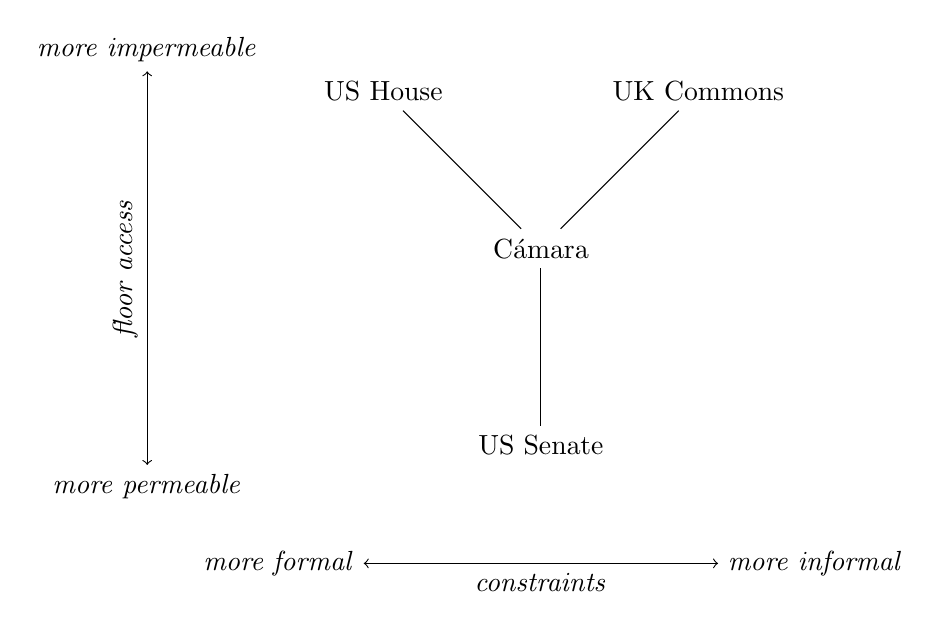
\begin{tikzpicture}
      \node at (-2, 2) {US House};
      \node at ( 2, 2) {UK Commons};
      \node at ( 0, 0) {Cámara};
      \node at ( 0,-2.5) {US Senate};
      \draw (-.25, .25) -- (-1.75, 1.75);
      \draw ( .25, .25) -- ( 1.75, 1.75);
      \draw (0,   -.25) -- ( 0,   -2.25);
      \draw[<->] (-2.25,-4) node[left] {\emph{more formal}} -- node[below] {\emph{constraints}} (2.25,-4) node[right] {\emph{more informal}};
      \draw[<->] (-5,-2.75) node[below] {\emph{more permeable}} -- node[sloped,above] {\emph{floor access}} (-5,2.25) node[above] {\emph{more impermeable}};
%      \draw[<->] (-5,-2.75) node[below] {\emph{less restrictive}} -- (-5,2.25) node[above] {\emph{more restrictive}};
    \end{tikzpicture}  
%% \caption{Formal and informal restrictions to members' legislative rights}\label{F:comparison}
%% \end{figure}



\end{document}

